
大多数人,都会以有组织的方式组织他们的软件项目。组织是方法和过程(如面向对象(OO)设计、编程语言规则、个人偏好、习惯或由项目规则规定的)的积极副作用。虽然规则和约定往往很无聊,但遵守它们会使项目结构更容易理解,有条理的材料对人类和计算机的感知都更好。当程序、规则、秩序和组织存在时,计算机可以对其进行理解。文档生成软件正是利用了这一点。

现在将介绍C和C++编程语言中最著名的文档生成软件之一:Doxygen。我们将学习如何将Doxygen与CMake集成,以自动生成CMake项目的文档。

接下来,先来了解一下Doxygen。

\subsubsubsection{6.2.1\hspace{0.2cm}了解Doxygen}

Doxygen是一个非常流行的C++项目文档软件,允许从代码生成文档。Doxygen理解C和C++语法,能够以编译器能够看到的方式看到代码结构。这允许Doxygen深入到软件项目的结构中,查看所有的类定义、命名空间、匿名函数、封装、变量、继承关系等。Doxygen将这些信息与开发者编写的内联代码文档结合起来。最终的结果是生成可读的各种文档,其兼容在线和离线阅读。

但\textit{天下没有免费的午餐}。为了能够理解代码注释,Doxygen要求注释采用预定义的一组格式。为了不分散本章的重点,请查看\url{https://www.doxygen.nl/manual/docblocks.html},找出与Doxygen兼容的注释格式。我们将在示例中使用Javadoc风格的注释。这里提供了一个C++函数的Javadoc注释示例:

\begin{lstlisting}[style=styleCXX]
/**
* Does foo with @p bar and @p baz
*
* @param [in] bar Level of awesomeness
* @param [in] baz Reason of awesomeness
*/
void foo(int bar, const char* baz){}
\end{lstlisting}

Doxygen还需要一个Doxyfile,其包含文档生成的所有参数,比如输出格式、排除的文件模式、项目名称等。因为配置参数太多,开始配置Doxygen可能会让人望而生畏,但CMake也自动生成一个Doxyfile。

随着我们深入了解,将了解为项目使用文档生成软件的好处。通过这种方式,使文档与代码保持一致变得更加容易,而且读取代码结构的能力也使绘图更加容易。

理论到此为止。让我们开始使用Doxygen和CMake。

\subsubsubsection{6.2.2\hspace{0.2cm}使用Doxygen和CMake}

CMake是一个面向C++的构建系统生成器,对集成C++项目中常用的外部工具有很好的支持。将Doxygen与CMake整合起来非常简单。我们将使用FindDoxygen.cmake将Doxygen集成到我们的项目中。默认情况下,该模块由CMake安装提供,不需要额外设置。

FindDoxygen.cmake是一个指定由\texttt{find\_package()}使用的模块包文件。主要用途是在环境中定位Doxygen,并提供一些额外的实用功能,以支持在CMake项目中生成文档。为了说明Doxygen的能力,本节将遵循第6章-示例01的示例。目标是为一个简单的计算器库,及其README文件生成文档。库的接口定义:

\begin{lstlisting}[style=styleCXX]
class calculator : private calculator_interface {
public:
	/**
	* Calculate the sum of two numbers, @p augend lhs and
	@p addend
	*
	* @param [in] augend The number to which @p addend is
	added
	* @param [in] addend The number which is added to
	@p augend
	*
	* @return double Sum of two numbers, @p lhs and @p rhs
	*/
	virtual double sum(double augend, double addend)
	override;
	/**
	* Calculate the difference of @p rhs from @p lhs
	*
	* @param [in] minuend The number to which @p
	subtrahend is subtracted
	* @param [in] subtrahend The number which is to be
	subtracted from @p minuend
	*
	* @return double Difference of two numbers, @p minuend
	and @p subtrahend
	*/
	virtual double sub(double minuend, double subtrahend)
	override;
	/*...*/
}; // class calculator
\end{lstlisting}

calculator类实现了在calculator\_interface类中定义的类接口,以Javadoc格式进行了正确的文档记录。我们期望Doxygen为calculator和calculator\_interface类生成应用程序编程接口(API)文档,以及继承图。类定义在calculator.hpp文件中,可以在chapter6/ex01\_doxdocgen目录的include/chapter6/ex01子目录下找到。另外,这里有一个名为README.md的Markdown文件。在chapter6/ex01\_doxdocgen目录中这包含了关于示例项目布局的基本信息,我们希望这个文件成为文档的主页。输入材料准备好后,通过检查示例的CMakeLists.txt文件也就是chapter6/ex01\_doxdocgen/CMakeLists.txt来进一步深入这个示例。CMakeLists.txt文件从寻找Doxygen包开始,如下所示:

\begin{lstlisting}[style=styleCMake]
find_package(Doxygen)
set(DOXYGEN_OUTPUT_DIRECTORY"${CMAKE_CURRENT_BINARY_DIR}/docs")
set(DOXYGEN_GENERATE_HTML YES)
set(DOXYGEN_GENERATE_MAN YES)
set(DOXYGEN_MARKDOWN_SUPPORT YES)
set(DOXYGEN_AUTOLINK_SUPPORT YES)
set(DOXYGEN_HAVE_DOT YES)
set(DOXYGEN_COLLABORATION_GRAPH YES)
set(DOXYGEN_CLASS_GRAPH YES)
set(DOXYGEN_UML_LOOK YES)
set(DOXYGEN_DOT_UML_DETAILS YES)
set(DOXYGEN_DOT_WRAP_THRESHOLD 100)
set(DOXYGEN_CALL_GRAPH YES)
set(DOXYGEN_QUIET YES)
\end{lstlisting}

\texttt{find\_package(…)}将使用FindDoxygen.cmake安装提供的cmake模块,以便在环境中查找Doxygen(如果存在的话)。省略REQUIRED参数是为了允许包维护人员打包项目而不需要安装,这可以确保在他们的环境中找到Doxygen,然后再进行下一步。接下来的几行设置了几个Doxygen配置。这些配置将存在由CMake生成的Doxyfile中。下面列出了每个选项的说明:

\begin{itemize}
\item 
DOXYGEN\_OUTPUT\_DIRECTORY: 设置Doxygen的输出目录。

\item 
DOXYGEN\_GENERATE\_HTML: 生成超文本标记语言(HTML)。

\item 
DOXYGEN\_GENERATE\_MAN: 生成MAN页面。

\item 
DOXYGEN\_AUTOLINK\_SUPPORT: 允许Doxygen自动链接语言符号和文件名到相关文档页面(若可用)。

\item 
DOXYGEN\_HAVE\_DOT: Doxygen环境有可用的dot,该命令可用于生成图像。这将使Doxygen能够使用依赖关系图、继承图和协作图来丰富生成的文档。

\item 
DOXYGEN\_COLLABORATION\_GRAPH: 为类生成协作图。

\item 
DOXYGEN\_CLASS\_GRAPH: 生成类图。

\item 
DOXYGEN\_UML\_LOOK: Instructs 生成类似统一建模语言(UML)的图。

\item 
DOXYGEN\_DOT\_UML\_DETAILS: 将类型和参数信息添加到UML图中。

\item 
DOXYGEN\_DOT\_WRAP\_THRESHOLD: 为UML图设置行换行阈值。

\item 
DOXYGEN\_CALL\_GRAPH: 为函数文档中的函数生成调用图。

\item 
DOXYGEN\_QUIET: 静默生成到标准输出(stdout)的Doxygen输出。
\end{itemize}

Doxygen的选项相当广泛,提供了更多的选项。若想进一步定制文档生成,请查看可以在Doxyfiles中使用的完整参数列表,网址是\url{https://www.doxygen.nl/manual/config.html}。要在CMake中设置Doxygen选项,在变量名前加上Doxygen\_并使用\texttt{set()}设置所需的值就好。写好旁注后,回到示例代码。前面显示的CMake代码后面跟着目标声明。以下代码行定义了一个静态库,其中包含了文档的示例代码:

\begin{lstlisting}[style=styleCMake]
add_library(ch6_ex01_doxdocgen_lib STATIC)
target_sources(ch6_ex01_doxdocgen_lib PRIVATE src/calculator.cpp)
target_include_directories(ch6_ex01_doxdocgen_lib PUBLIC include)
target_compile_features(ch6_ex01_doxdocgen_lib PRIVATE cxx_std_11)
\end{lstlisting}

随后,以下代码行定义了一个使用前面定义的静态库目标的可执行文件:

\begin{lstlisting}[style=styleCMake]
add_executable(ch6_ex01_doxdocgen_exe src/main.cpp)
target_compile_features(ch6_ex01_doxdocgen_exe PRIVATE cxx_std_11)
target_link_libraries(ch6_ex01_doxdocgen_exe PRIVATE ch6_ex01_doxdocgen_lib)
\end{lstlisting}

最后,使用\texttt{doxygen\_add\_docs(…)}来指定希望生成文档的代码:

\begin{lstlisting}[style=styleCMake]
doxygen_add_docs(
	ch6_ex01_doxdocgen_generate_docs
	"${CMAKE_CURRENT_LIST_DIR}"
	ALL
	COMMENT "Generating documentation for Chapter 6 - Example
		01 with Doxygen"
)
\end{lstlisting}
 
\texttt{doxygen\_add\_docs(…)}由FindDoxygen.cmake模块提供。其唯一目的是提供一种方便的方法来为文档生成创建CMake目标,\texttt{doxygen\_add\_docs(…)}函数的签名显示在这里(省略不相关的参数):

\begin{lstlisting}[style=styleCMake]
doxygen_add_docs(targetName
	[filesOrDirs...]
	[ALL]
	[COMMENT comment])
\end{lstlisting}

第一个参数targetName是文档目标的名称,该函数将生成一个名为targetName的自定义目标。这个目标将触发Doxygen,并在构建时从代码创建文档。下一个参数列表filesOrDirs,是包含想要从文档生成的代码的文件或目录的列表。ALL参数用于使CMake的ALL元目标依赖于\texttt{doxygen\_add\_docs(…)}创建的文档目标,因此在构建ALL元目标时自动触发文档生成。最后,COMMENT参数用于让CMake在构建目标时输出一条消息。COMMENT主要用于诊断目的,以便快速知道是否生成了文档。

对\texttt{doxygen\_add\_docs(…)}进行了简短的介绍之后,回到示例代码,并解释\texttt{doxygen\_add\_docs(…)}在场景中做了什么。其创建了一个名为ch6\_ex01\_doxdocgen\_generate\_docs的目标,将\$\{CMAKE\_CURRENT\_LIST\_DIR\}添加到文档生成目录,请求ALL元目标依赖于它,并指定在构建目标时打印COMMENT参数。

好了,是时候测试一下这个是否有效了。进入chapter\_6/目录,在build/目录中使用以下命令配置项目:

\begin{tcblisting}{commandshell={}}
cd chapter_6/
cmake –S . -B build/
\end{tcblisting}

检查CMake输出,查看配置是否成功。若配置成功,CMake成功地在环境中找到了Doxygen。应该可以在CMake的输出中看到:

\begin{tcblisting}{commandshell={}}
Found Doxygen: /usr/bin/doxygen (found version "1.9.1")
    found components: doxygen dot
\end{tcblisting}

成功配置之后,尝试使用以下命令构建:

\begin{tcblisting}{commandshell={}}
cmake --build build/
\end{tcblisting}

构建输出中,应该能够看到提供给COMMENT参数的文在CMake输出中,所以文档目标正在构建,Doxygen正在运行。注意,这里没有为CMake构建命令指定-{}-target参数,这将直接构建ALL元目标。由于我们已经将ALL参数赋给了\texttt{doxygen\_add\_docs(…)},因此也构建了一个ch6\_ex01\_doxdocgen\_generate\_docs目标。build命令的输出应该类似于这样:

\begin{tcblisting}{commandshell={}}
[ 20%] Generating documentation for Chapter 6 - Example 01
with Doxygen
Doxygen version used: 1.9.1
Searching for include files...
Searching for example files...
/*…*/
Running dot...
Running dot for graph 1/1
lookup cache used 9/65536 hits=13 misses=9
finished...
[ 20%] Built target ch6_ex01_doxdocgen_generate_docs
[ 40%] Building CXX object ex01_doxdocgen/CmakeFiles
  /ch6_ex01_doxdocgen_lib.dir/src/calculator.cpp.o
[ 60%] Linking CXX static library
libch6_ex01_doxdocgen_lib.a
[ 60%] Built target ch6_ex01_doxdocgen_lib
[ 80%] Building CXX object ex01_doxdocgen/CmakeFiles
  /ch6_ex01_doxdocgen_exe.dir/src/main.cpp.o
[100%] Linking CXX executable ch6_ex01_doxdocgen_exe
[100%] Built target ch6_ex01_doxdocgen_exe
\end{tcblisting}

我们已经成功地构建了项目和文档,检查一下在\$\{CMAKE\_CURRENT\_BINARY\_DIR\}/docs输出文件夹中生成的文档:

\begin{tcblisting}{commandshell={}}
14:27 $ ls build/ex01_doxdocgen/docs/
html man
\end{tcblisting}

这里,可以看到Doxygen将HTML和MAN页面输出发送到html/和man/目录中,检查每种类型的最终结果。要检查生成的MAN页面,只需输入以下命令:

\begin{lstlisting}[style=styleCMake]
man build/ex01_doxdocgen/docs/man/man3
	/chapter6_ex01_calculator.3
NAME
		chapter6::ex01::calculator - The 'calculator' class
		  interface.
SYNOPSIS
		#include <calculator.hpp>
	Static Public Member Functions
		static double sum (double augend, double addend)
		static double sub (double minuend, double
			subtrahend)
		static double mul (double multiplicand, double
			multiplier)
		static double div (double dividend, double divisor)
Detailed Description
		The 'calculator' class interface.
Member Function Documentation
	double chapter6::ex01::calculator::div (double
		dividend, double divisor) [static]
			Divide dividend with divisor
			Parameters
				dividend The number to be divided by divisor
				divisor The number by which divisor is to be
					divided
			Returns
				double Quotient of two numbers, dividend and
					divisor
Manual page chapter6_ex01_calculator.3 line 1 (press h for
	help or q to quit)
\end{lstlisting}

太棒了!代码注释变成了MAN页面。同样,查一下HTML输出。使用您选择的浏览器打开build/ex01\_doxdocgen/docs/html/index.html文件:

\begin{tcblisting}{commandshell={}}
google-chrome build/ex01_doxdocgen/docs/html/index.html
\end{tcblisting}

这将显示文档的主页面,如下图所示:

\begin{center}
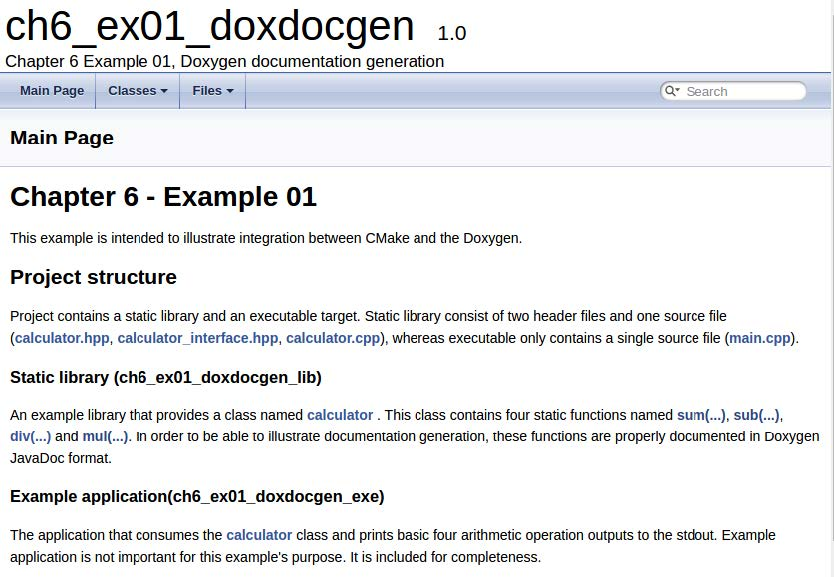
\includegraphics[width=0.6\textwidth]{content/2/chapter6/images/1.jpg}\\
图6.1 文档的主页
\end{center}

可以看到Doxygen渲染了README.md Markdown文件内容到主页。注意,主页只是作为示例提供的。Doxygen可以在生成的文档中嵌入任意数量的Markdown文件,甚至可以用到相关文档的链接替换了文件名、类名和函数名。这是通过Doxygen的AUTOLINK特性和@ref指令实现的。单击主页面的静态库部分下面的calculator链接,以访问calculator 类的API文档。calculator类文档页面应该如下所示:

\begin{center}
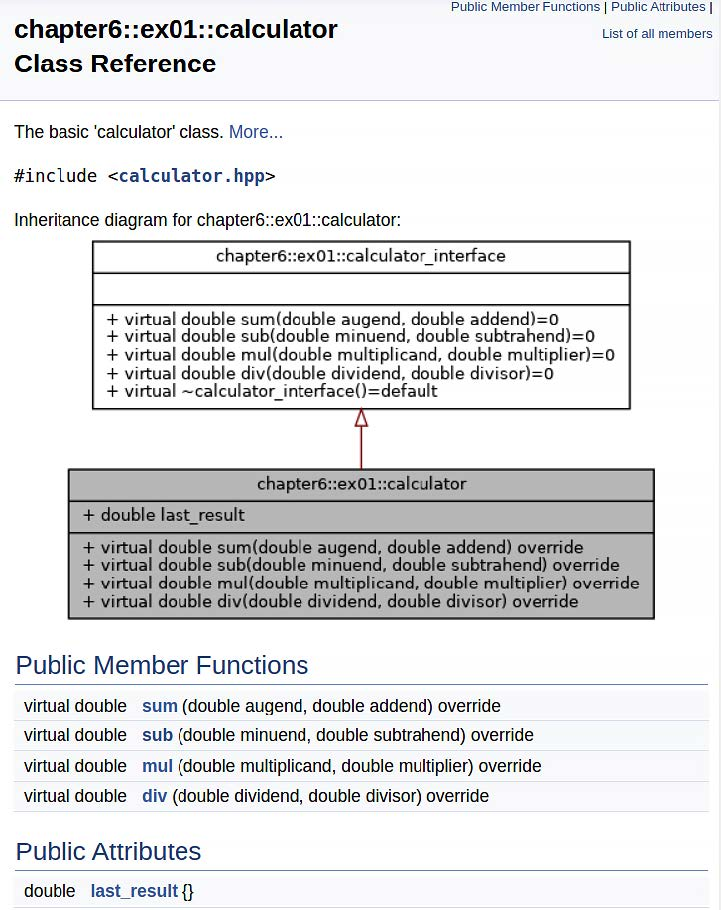
\includegraphics[width=0.7\textwidth]{content/2/chapter6/images/2.jpg}\\
图6.2 为计算器类生成的HTML文档(基本布局)
\end{center}

可以看到Doxygen知道计算器类继承自calculator\_interface,并为calculator类绘制了继承图。

\begin{tcolorbox}[colback=webgreen!5!white,colframe=webgreen!75!black,title=Note]
Doxygen需要dot工具来渲染图表,dot在Graphviz软件包中。
\end{tcolorbox}

此外,生成的图包含UML样式的函数名和封装符号。下图显示了详细的成员函数文档:

\begin{center}
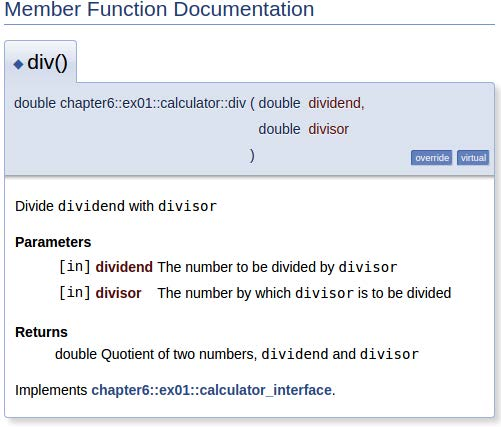
\includegraphics[width=0.6\textwidth]{content/2/chapter6/images/3.jpg}\\
图6.3 为calculator类的div()函数生成的文档
\end{center}

如图6.3所示,Doxygen在将内容放入清晰易读的布局方面做得很好。最后,导航到Files | File List | main.cpp,查看main.cpp的文档,以说明依赖关系图是什么样子的。可以在下面的截图中看到文档页面的表示形式:

\begin{center}
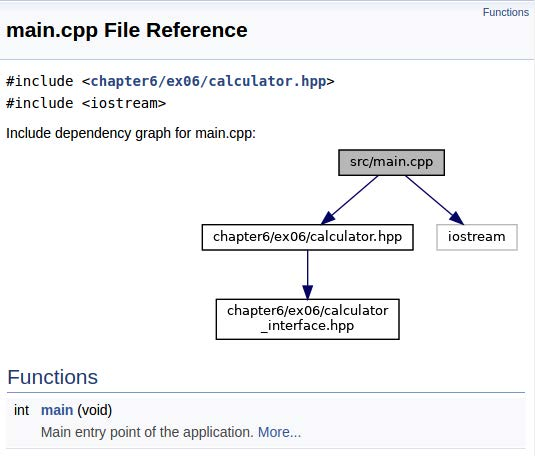
\includegraphics[width=0.6\textwidth]{content/2/chapter6/images/4.jpg}\\
图6.4  main.cpp文档页面
\end{center}

从上图的依赖关系图可以看出,main.cpp文件直接依赖于iostream和chapter6/ex06/calculator.hpp文件,间接依赖于chapter6/ex06/calculator\_interface.hpp文件。文档中提供依赖性信息非常有用,使用者将确切地知道文件依赖关系是什么,而不必深入到代码中。若再向下滚动一点,也会看到main()函数的调用图,如下图所示:

\begin{center}
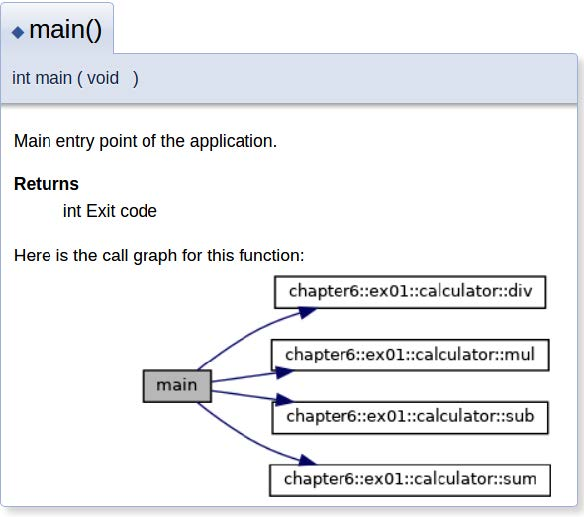
\includegraphics[width=0.6\textwidth]{content/2/chapter6/images/5.jpg}\\
图6.5  main()函数的调用图
\end{center}

我们用不到20行额外的CMake代码,为我们的代码生成了两种不同格式的图表文档。多酷啊!现在,有了这种能力,就很难找到借口来避免文档化,但这一章的旅程还没有结束。接下来的部分会将定制的UML图嵌入到文档中来丰富我们的知识。来一起看看吧!
 
\subsubsubsection{6.2.3\hspace{0.2cm}将UML图嵌入到文档中}

前一节中,学习了如何利用Doxygen为CMake项目生成图表和文档,但是并不是每个图表都可以从代码中推断出来。我们可能需要绘制自定义图,来说明实体与代码上下文中不可用的外部系统之间的关系。要解决这个问题,需要在代码或注释中提供该上下文,以便再次使用文档生成。如预期的那样,这可以通过Doxygen实现。Doxygen允许将PlantUML图表嵌入到注释中,这使我们能够绘制PlantUML支持的任何图表。但在开始将PlantUML代码放入Doxygen注释前,有一件事必须注意:在Doxygen中需要启用PlantUML支持。

在Doxygen中启用PlantUML支持非常简单。Doxygen需要将PLANTUML\_JAR\_PATH变量设置为PLANTUML.jar文件的位置,所以得找出那个文件的位置。可以使用\texttt{find\_path(…)},\texttt{find\_path(…)}和\texttt{find\_program(…)}类似,指定用于定位文件的路径。使用本节第6章-例02,让我们深入到示例代码的CMakeLists文件中,它位于chapter\_6/ex02\_doxplantuml/CMakeLists.txt。让我们从\texttt{find\_path(…)}开始看:

\begin{lstlisting}[style=styleCMake]
find_path(PLANTUML_JAR_PATH NAMES plantuml.jar HINTS
	"/usr/share/plantuml" REQUIRED)
find_package(Doxygen REQUIRED)
set(DOXYGEN_OUTPUT_DIRECTORY "${CMAKE_CURRENT_BINARY_DIR}
	/docs")
set(DOXYGEN_GENERATE_HTML YES)
set(DOXYGEN_AUTOLINK_SUPPORT YES)
set(DOXYGEN_PLANTUML_JAR_PATH "${PLANTUML_JAR_PATH}")
set(DOXYGEN_QUIET YES)
\end{lstlisting}

\texttt{find\_path(…)}的输出为PLANTUML\_JAR\_PATH。NAMES是搜索位置中的文件名。HINTS是默认搜索位置之外的路径,这对于在非标准位置很有用。最后,REQUIRED参数用于使plantuml.jar必须找到,因此当无法找到plantuml.jar时,CMake将失败并退出。下面的Doxygen配置部分与我们之前的示例(第6章-示例01)完全相同,不同的是将DOXYGEN\_PLANTUML\_JAR\_PATH设置为找到的PlantUML目录路径。此外,本例中不需要的变量也会省略了。Doxygen现在应该可以使用PlantUML了。我们用一个PlantUML示例图进行测试,将其嵌入到src/main.cpp源文件中:

\begin{lstlisting}[style=styleCXX]
/**
* @brief Main entry point of the application
  @startuml{system_interaction.png} "System Interaction
    Diagram"
  user -> executable : main()
  user -> stdin
  executable -> executable: read_stdin()
  executable -> stdout
  @enduml
* @return int Exit code
*/
int main(void) {
	std::cout << "Greetings from the echo application!" <<
	std::endl;
	std::string input;
	while (std::getline(std::cin, input)) {
		std::cout << input;
	}
}
\end{lstlisting}

@startuml和@enduml Doxygen注释关键字分别用于指示PlantUML图的开始和结束。普通的PlantUML代码可以放在@startuml - @enduml块中。我们的示例中,有一个简单的应用程序系统交互图。若一切按计划进行,应该在main()函数的文档中看到嵌入的PlantUML图。可以用下面所示的代码构建示例来生成文档:
 
\begin{tcblisting}{commandshell={}}
cd chapter_6/
cmake -S ./ -B build/
cmake --build build/
\end{tcblisting}

第二个示例的文档现在构建好了。使用浏览器打开生成的build/ex02\_doxplantuml/docs/html/index.html html文档,运行以下命令:

\begin{tcblisting}{commandshell={}}
google-chrome build/ex02_doxplantuml/docs/html/index.html
\end{tcblisting}

会有以下输出:

\begin{center}
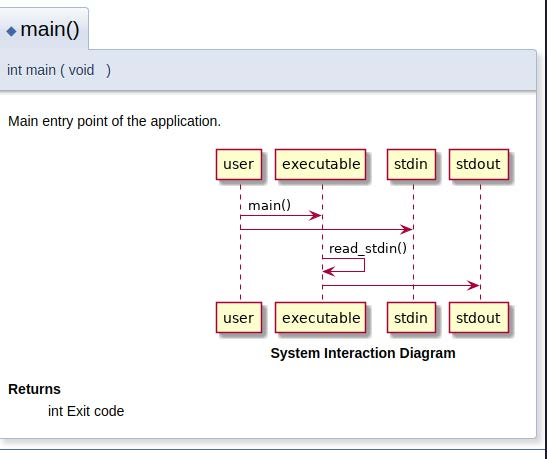
\includegraphics[width=0.6\textwidth]{content/2/chapter6/images/6.jpg}\\
图6.6  main()函数文档中嵌入PlantUML图
\end{center}

图6.6中,可以看到Doxygen生成了PlantUML图,并将其嵌入到文档中。现在,就可以将自定义图嵌入到生成的文档中了,这允许我们解释复杂的系统和关系,而不必与外部绘图工具进行交互。

我们有了生成文档的正确工具,是时候学习如何打包和交付文档了。下一节中,我们将学习交付文档的方法以及所涉及的软件。








